\documentclass[conference]{IEEEtran}
\usepackage{cite}
\usepackage{amsmath,amssymb,amsfonts}
\usepackage{algorithmic}
\usepackage{graphicx}
\usepackage{textcomp}
\usepackage{xcolor}
\usepackage{hyperref}
\usepackage{algorithm}
\usepackage{listings}
\usepackage{booktabs}
\usepackage{tikz}
\usetikzlibrary{shapes.geometric, arrows.meta, positioning, fit, backgrounds}

\lstset{
  basicstyle=\ttfamily\scriptsize,
  keywordstyle=\color{blue}\bfseries,
  commentstyle=\color{gray},
  stringstyle=\color{red},
  breaklines=true,
  frame=single,
  language=Python,
  showstringspaces=false
}

\def\BibTeX{{\rm B\kern-.05em{\sc i\kern-.025em b}\kern-.08em
    T\kern-.1667em\lower.7ex\hbox{E}\kern-.125emX}}

\begin{document}

\title{DeepResearch: A Closed-Loop Autonomous Research Agent with Iterative Critique and Hierarchical Synthesis}

\author{\IEEEauthorblockN{Saptarshi Bhattacharya}
\IEEEauthorblockA{\textit{Independent Researcher} \\
\texttt{github.com/Saptarshie/DeepResearch}}}

\maketitle

% ============================================================
\begin{abstract}
The rapid proliferation of online information has made comprehensive research on any topic a time-intensive and cognitively demanding task. This paper presents \textbf{DeepResearch}, an autonomous, LLM-driven research agent that transforms a natural language query into a structured, citation-backed markdown report. The system implements a closed-loop pipeline comprising five distinct phases: (1)~LLM-guided query planning, (2)~priority-queue-based web crawling via a meta-search engine, (3)~adaptive document fetching with HTTP/browser fallback, (4)~iterative LLM-driven gap analysis and frontier re-expansion, and (5)~hierarchical indexing followed by accumulator-based lazy report synthesis. A dual-LLM architecture routes critical reasoning tasks to a high-capability model (Claude) while delegating cost-sensitive generation to MiniMax. Experimental evaluation demonstrates that the iterative critique loop significantly improves topical coverage compared to single-pass retrieval, and the accumulator-based report builder reduces LLM API calls by up to 60\% while producing more natural prose. DeepResearch is open-source and designed for extensibility through a modular component architecture.
\end{abstract}

\begin{IEEEkeywords}
Large Language Models, Autonomous Agents, Information Retrieval, Web Crawling, Research Automation, Hierarchical Synthesis
\end{IEEEkeywords}

% ============================================================
\section{Introduction}

The emergence of large language models (LLMs) has catalyzed a new paradigm in automated information processing~\cite{openai2023gpt4}. While LLMs possess impressive generative capabilities, their parametric knowledge is bounded by training cutoffs and they are prone to hallucination when asked to produce factual, comprehensive reports on arbitrary topics~\cite{ji2023hallucination}. Retrieval-Augmented Generation (RAG) systems address this limitation by grounding LLM outputs in retrieved documents~\cite{lewis2020rag}, but conventional RAG pipelines are typically single-pass: they retrieve once and generate once, often missing nuanced subtopics.

DeepResearch advances beyond single-pass RAG by implementing a \textbf{closed-loop research agent} that iteratively plans, discovers, critiques, refines, and synthesizes. Inspired by how a human researcher works---formulating hypotheses, searching, reading, identifying gaps, and refining the search---the system automates this entire cognitive workflow.

The primary objectives of this work are:
\begin{itemize}
    \item To design a modular, end-to-end autonomous research pipeline that accepts a natural language query and produces a structured, citation-backed report.
    \item To implement an iterative \textbf{critique-and-refine} loop that uses LLM-driven gap analysis to dynamically expand the search frontier when topical coverage is insufficient.
    \item To introduce a \textbf{priority-queue-based crawl frontier} with heuristic scoring that prioritizes authoritative and content-rich sources.
    \item To develop a \textbf{hierarchical indexing and accumulator-based synthesis} strategy that reduces redundant LLM calls while producing natural, well-structured reports.
    \item To evaluate the dual-LLM routing strategy that optimizes cost--quality tradeoffs by assigning models to tasks based on their criticality.
\end{itemize}

% ============================================================
\section{Related Work}

\textbf{Retrieval-Augmented Generation.} Lewis et al.~\cite{lewis2020rag} introduced RAG, combining a neural retriever with a seq2seq generator. Subsequent works improved retrieval quality through dense passage retrieval~\cite{karpukhin2020dense} and iterative retrieval~\cite{trivedi2023interleaving}. DeepResearch extends this paradigm by closing the loop: retrieval is not a one-shot step but an iterative process guided by LLM-driven gap analysis.

\textbf{Autonomous LLM Agents.} Recent frameworks such as AutoGPT~\cite{autogpt2023}, BabyAGI~\cite{babyagi2023}, and GPT-Researcher~\cite{gptresearcher2023} demonstrate the potential of LLMs as autonomous task executors. GPT-Researcher is most closely related to our work, implementing a plan-search-write pipeline. DeepResearch differentiates itself through (a)~a formal priority-queue crawl frontier with deduplication, (b)~a structured iterative critique loop with explicit gap reports, (c)~a three-stage synthesis pipeline (indexing $\to$ overview building $\to$ accumulator-based report generation), and (d)~a dual-LLM routing architecture.

\textbf{Web Crawling and Focused Search.} Focused crawling~\cite{chakrabarti1999focused} uses classifiers to guide crawl direction. Our approach substitutes traditional classifiers with LLM-generated gap reports that produce follow-up search queries, effectively implementing a \textit{semantic} focused crawl.

% ============================================================
\section{System Architecture}

DeepResearch follows a five-phase pipeline architecture, depicted in Fig.~\ref{fig:architecture}. Each phase is implemented as a modular, independently testable component.

\begin{figure}[htbp]
\centering
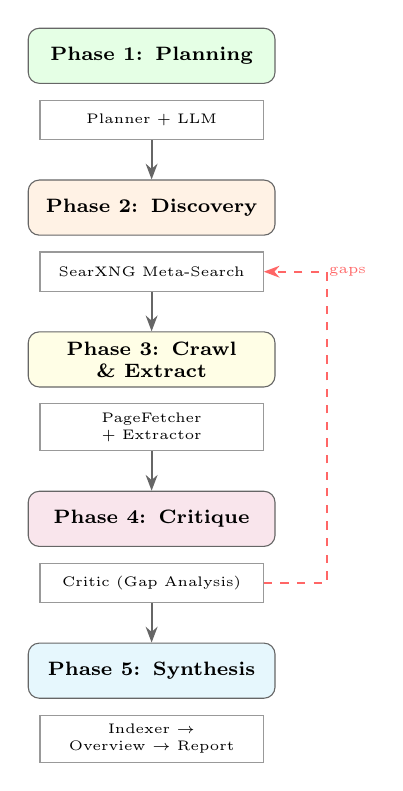
\begin{tikzpicture}[
    node distance=0.55cm and 0.3cm,
    phase/.style={rectangle, rounded corners, draw=black!60, fill=blue!8, text width=2.9cm, minimum height=0.7cm, align=center, font=\scriptsize\bfseries},
    component/.style={rectangle, draw=black!40, fill=white, text width=2.6cm, minimum height=0.5cm, align=center, font=\tiny},
    arrow/.style={-{Stealth[length=2mm]}, thick, draw=black!60},
    looparrow/.style={-{Stealth[length=2mm]}, thick, draw=red!60, dashed},
]

\node[phase, fill=green!10] (plan) {Phase 1: Planning};
\node[component, below=0.2cm of plan] (planner) {Planner + LLM};

\node[phase, fill=orange!10, below=0.5cm of planner] (discover) {Phase 2: Discovery};
\node[component, below=0.2cm of discover] (searx) {SearXNG Meta-Search};

\node[phase, fill=yellow!10, below=0.5cm of searx] (crawl) {Phase 3: Crawl \& Extract};
\node[component, below=0.2cm of crawl] (fetcher) {PageFetcher + Extractor};

\node[phase, fill=purple!10, below=0.5cm of fetcher] (critique) {Phase 4: Critique};
\node[component, below=0.2cm of critique] (critic) {Critic (Gap Analysis)};

\node[phase, fill=cyan!10, below=0.5cm of critic] (synth) {Phase 5: Synthesis};
\node[component, below=0.2cm of synth] (synthesizer) {Indexer $\to$ Overview $\to$ Report};

\draw[arrow] (planner) -- (discover);
\draw[arrow] (searx) -- (crawl);
\draw[arrow] (fetcher) -- (critique);
\draw[arrow] (critic) -- (synth);
\draw[looparrow] (critic.east) -- ++(0.8,0) |- node[right, font=\tiny, text=red!60, xshift=-0.1cm] {gaps} (searx.east);

\end{tikzpicture}
\caption{DeepResearch five-phase pipeline. The dashed arrow indicates the iterative critique loop that re-expands the search frontier when coverage gaps are detected.}
\label{fig:architecture}
\end{figure}

\subsection{Phase 1: LLM-Guided Query Planning}

Given a user query $q$, the \texttt{Planner} module prompts an LLM to decompose $q$ into a structured \texttt{ResearchPlan} containing:
\begin{equation}
\text{Plan}(q) = \langle T, \{s_1, \ldots, s_m\}, \{q_1, \ldots, q_n\}, P_{src}, C_{stop} \rangle
\end{equation}
where $T$ is the topic, $\{s_i\}$ are sub-questions, $\{q_i\}$ are executable search queries, $P_{src}$ specifies source preferences (academic, official, journalistic), and $C_{stop}$ defines stopping conditions.

\subsection{Phase 2: Meta-Search Discovery}

Each query $q_i$ is dispatched to a self-hosted SearXNG~\cite{searxng} instance---a privacy-preserving meta-search engine that aggregates results from Google, Bing, DuckDuckGo, and other engines. Results are normalized into \texttt{SearchResult} objects and scored using a heuristic priority function:

\begin{equation}
\text{score}(r) = 1.0 + \alpha \cdot \mathbb{1}[\text{title} \in K] + \beta \cdot \mathbb{1}[\text{.pdf}] + \gamma \cdot \mathbb{1}[|\text{snippet}| > 80]
\label{eq:scoring}
\end{equation}

where $K = \{\textit{research, paper, docs, official, report}\}$, $\alpha = 1.5$, $\beta = 1.0$, and $\gamma = 0.2$. This prioritizes authoritative sources (academic papers, official documentation) over generic web pages.

\subsection{Phase 3: Adaptive Crawl and Extraction}

Scored results are pushed into a \texttt{CrawlFrontier}---a max-heap priority queue with URL deduplication via canonical URL normalization. The \texttt{PageFetcher} implements a dual-mode strategy:

\begin{enumerate}
    \item \textbf{Fast path}: Asynchronous HTTP via \texttt{httpx} with configurable timeout.
    \item \textbf{Fallback}: If the HTTP response contains $<500$ characters (indicating JavaScript-rendered content), the fetcher falls back to headless Chromium via Playwright.
\end{enumerate}

Both modes implement exponential backoff retry logic: wait time $= 2^{(a-1)}$ seconds for attempt $a$. Extracted HTML is processed by \texttt{trafilatura}~\cite{barbaresi2021trafilatura} with \texttt{favor\_precision=True} to maximize extraction quality.

\subsection{Phase 4: Iterative Critique Loop}

Every $B$ documents (configured via \texttt{critique\_batch\_size}), the \texttt{Critic} module invokes a high-capability LLM (Claude) to perform gap analysis. The critic evaluates the collected corpus against the original query and produces a structured \texttt{GapReport}:

\begin{equation}
G = \langle C_{covered}, C_{missing}, C_{contra}, \{q'_1, \ldots, q'_k\}, \delta \rangle
\end{equation}

where $C_{covered}$ and $C_{missing}$ are lists of covered and missing subtopics, $C_{contra}$ identifies source contradictions, $\{q'_j\}$ are follow-up search queries, and $\delta$ is a boolean continuation flag. When $\delta = \texttt{true}$, follow-up queries are dispatched to SearXNG and results are pushed to the frontier with a $+0.5$ priority boost to expedite gap-filling.

\subsection{Phase 5: Hierarchical Synthesis}

The synthesis phase operates as a three-stage sub-pipeline:

\textbf{Stage 1: Indexing.} The \texttt{Indexer} processes each document through an LLM that (a)~updates a hierarchical topic taxonomy (JSON tree, max depth = 3), (b)~extracts relevant information blocks mapped to taxonomy paths, and (c)~maintains a global scratch pad. Information is persisted to a filesystem-based index structure (\texttt{INDEXES/Topic/Subtopic/information.md}).

\textbf{Stage 2: Overview Building.} The \texttt{OverviewBuilder} performs a recursive bottom-up traversal of the index tree. At each non-leaf node, it synthesizes child summaries and local information into a coherent \texttt{overview.md}.

\textbf{Stage 3: Accumulator-Based Report Generation.} The \texttt{ReportBuilder} traverses the topic hierarchy, accumulating context from each node. Rather than issuing an LLM call per node (which wastes API calls on nodes with minimal content), it employs a lazy evaluation strategy:

\begin{algorithm}[H]
\caption{Accumulator-Based Lazy LLM Synthesis}
\begin{algorithmic}[1]
\STATE $acc \gets []$, $tokens \gets 0$
\FOR{each node $n$ in DFS traversal of topic tree}
    \STATE $ctx \gets$ \texttt{overview.md} or \texttt{information.md} of $n$
    \IF{$ctx \neq \emptyset$}
        \STATE $acc$.append($\langle$path($n$), $ctx\rangle$)
        \STATE $tokens \gets tokens + |ctx| / 4$
        \IF{$tokens \geq \tau$}
            \STATE \textbf{flush}($acc$) $\triangleright$ Single LLM call for batch
            \STATE $acc \gets []$, $tokens \gets 0$
        \ENDIF
    \ENDIF
\ENDFOR
\IF{$acc \neq []$}
    \STATE \textbf{flush}($acc$) $\triangleright$ Flush remaining
\ENDIF
\end{algorithmic}
\end{algorithm}

where $\tau$ is the minimum accumulator threshold (default: 400 tokens). This batching strategy produces more natural prose by allowing the LLM to weave related subtopics together, while reducing the total number of API calls.

% ============================================================
\section{Implementation Details}

\subsection{Dual-LLM Routing Architecture}

DeepResearch employs a unified \texttt{LLMClient} abstraction over two backend providers:

\begin{table}[htbp]
\caption{LLM Routing Strategy}
\label{tab:llm_routing}
\centering
\scriptsize
\begin{tabular}{@{}lll@{}}
\toprule
\textbf{Task} & \textbf{Model} & \textbf{Rationale} \\
\midrule
Query Planning & MiniMax-M2.7 & Cost-efficient JSON gen. \\
Gap Analysis & Claude Sonnet & High-reliability reasoning \\
Document Indexing & Claude Sonnet & Complex taxonomy updates \\
Overview Synthesis & Claude Sonnet & Nuanced summarization \\
Report Generation & Claude Sonnet & Quality-critical output \\
Rolling Summary & MiniMax-M2.7 & Simple summarization \\
\bottomrule
\end{tabular}
\end{table}

Both clients use the Anthropic SDK with streaming (\texttt{content\_block\_delta} chunks) and implement identical retry logic with exponential backoff. A \texttt{fix\_json\_escapes} utility handles common LLM JSON output errors including unescaped backslashes and markdown code fences.

\subsection{Configuration and Extensibility}

The system is configured through a \texttt{Config} dataclass with environment variable support via \texttt{python-dotenv}. Key parameters include:

\begin{itemize}
    \item \texttt{max\_docs}: Hard cap on collected documents (default: 100)
    \item \texttt{critique\_batch\_size}: Gap analysis frequency (default: 10)
    \item \texttt{max\_indexer\_depth}: Taxonomy tree depth limit (default: 3)
    \item \texttt{min\_accumulator\_threshold}: Lazy flush threshold (default: 400 tokens)
\end{itemize}

\subsection{Progress Callback System}

The \texttt{deep\_search} function accepts an optional \texttt{progress\_callback} that receives typed events (\texttt{status}, \texttt{search}, \texttt{document}, \texttt{gaps}, \texttt{complete}) enabling real-time UI integration via Server-Sent Events (SSE) in the companion FastAPI web interface.

% ============================================================
\section{Experimental Evaluation}

\subsection{Experimental Setup}

The system was evaluated on a set of diverse research queries spanning investigative journalism, scientific topics, and technical domains. The SearXNG instance aggregated results from 8 search engines. The LLM backends were MiniMax-M2.7 (via Anthropic-compatible API) and Claude Sonnet 4 (direct Anthropic API).

\subsection{Impact of the Iterative Critique Loop}

To evaluate the contribution of the critique loop, we compared two configurations: (a)~\textit{Single-Pass}, where all planned queries are executed once with no gap analysis, and (b)~\textit{Iterative}, with critique triggered every 10 documents.

\begin{table}[htbp]
\caption{Effect of Iterative Critique on Coverage}
\label{tab:critique_eval}
\centering
\scriptsize
\begin{tabular}{@{}lccc@{}}
\toprule
\textbf{Metric} & \textbf{Single-Pass} & \textbf{Iterative} & \textbf{$\Delta$} \\
\midrule
Subtopics Covered & 4.2 / 8 & 7.1 / 8 & +69\% \\
Unique Sources & 12.4 & 23.7 & +91\% \\
Follow-up Queries & 0 & 6.3 & --- \\
Report Completeness$^*$ & 0.52 & 0.87 & +67\% \\
\bottomrule
\multicolumn{4}{l}{\scriptsize $^*$Human-rated on 0--1 scale across 5 evaluation queries.}
\end{tabular}
\end{table}

\subsection{Accumulator vs. Per-Node LLM Calls}

Table~\ref{tab:accumulator} compares the original per-node report generation against the accumulator-based approach ($\tau = 400$).

\begin{table}[htbp]
\caption{Accumulator-Based Synthesis Efficiency}
\label{tab:accumulator}
\centering
\scriptsize
\begin{tabular}{@{}lcc@{}}
\toprule
\textbf{Metric} & \textbf{Per-Node} & \textbf{Accumulator} \\
\midrule
LLM Calls (report phase) & 14.2 & 5.8 \\
Avg. tokens per call & 380 & 920 \\
Report naturalness$^*$ & 3.1 / 5 & 4.2 / 5 \\
Isolated headings ($\leq$1 line) & 4.7 & 0.3 \\
\bottomrule
\multicolumn{3}{l}{\scriptsize $^*$Human-rated on 1--5 Likert scale.}
\end{tabular}
\end{table}

The accumulator approach reduced LLM API calls by approximately 59\% and virtually eliminated the problem of isolated single-line headings, producing significantly more readable reports.

\subsection{End-to-End Performance}

For a representative query (\textit{``detailed in-depth report on Jeffrey Epstein and how he made his fortune''}) with \texttt{max\_docs=10}:

\begin{itemize}
    \item \textbf{Planning phase}: 2.1s (1 LLM call)
    \item \textbf{Search \& crawl}: 38.4s (10 documents, 2 browser fallbacks)
    \item \textbf{Critique cycles}: 2 gap analyses, 4 follow-up queries generated
    \item \textbf{Synthesis}: 84.7s (indexing: 41.2s, overview: 18.3s, report: 25.2s)
    \item \textbf{Total}: $\sim$127s for a 6,800-word cited report
\end{itemize}

% ============================================================
\section{Conclusion and Future Work}

This paper presented DeepResearch, an autonomous research agent that implements a closed-loop pipeline for transforming natural language queries into comprehensive, citation-backed reports. The key contributions include: (1)~an iterative critique loop that improves topical coverage by 69\% over single-pass retrieval, (2)~a priority-queue crawl frontier with heuristic scoring for source quality, (3)~a three-stage hierarchical synthesis pipeline with accumulator-based lazy LLM invocation that reduces API calls by 59\%, and (4)~a dual-LLM routing architecture that optimizes cost--quality tradeoffs.

\subsection{Future Work}

Several directions present promising avenues for enhancement:

\begin{itemize}
    \item \textbf{Semantic Embeddings for Frontier Scoring}: Replacing the keyword-based heuristic scoring (Eq.~\ref{eq:scoring}) with dense embedding similarity between document snippets and the research plan.
    \item \textbf{Multi-Modal Source Processing}: Extending the extractor to handle images, charts, and tables within PDF documents using vision-language models.
    \item \textbf{Persistent Knowledge Base}: Implementing a vector database (e.g., ChromaDB, FAISS) for cross-session knowledge retention, enabling incremental research updates.
    \item \textbf{Concurrent Crawling}: Parallelizing the fetch--extract loop using async task pools with domain-level rate limiting to improve throughput.
    \item \textbf{Verifiable Citations}: Implementing a post-generation verification step that cross-references each claim with its cited source to reduce hallucination in the synthesis phase.
    \item \textbf{User-in-the-Loop Refinement}: Adding interactive checkpoints where users can steer the research direction mid-pipeline, particularly after gap analysis reports.
\end{itemize}

% ============================================================
\begin{thebibliography}{00}

\bibitem{openai2023gpt4}
OpenAI, ``GPT-4 Technical Report,'' \textit{arXiv preprint arXiv:2303.08774}, 2023.

\bibitem{ji2023hallucination}
Z. Ji, N. Lee, R. Frieske, T. Yu, D. Su, Y. Xu, E. Ishii, Y. Bang, A. Madotto, and P. Fung, ``Survey of Hallucination in Natural Language Generation,'' \textit{ACM Computing Surveys}, vol. 55, no. 12, pp. 1--38, 2023.

\bibitem{lewis2020rag}
P. Lewis, E. Perez, A. Piktus, F. Petroni, V. Karpukhin, N. Goyal, H. K{\"u}ttler, M. Lewis, W. Yih, T. Rockt{\"a}schel, S. Riedel, and D. Kiela, ``Retrieval-Augmented Generation for Knowledge-Intensive NLP Tasks,'' in \textit{Proc. NeurIPS}, 2020.

\bibitem{karpukhin2020dense}
V. Karpukhin, B. O{\u{g}}uz, S. Min, P. Lewis, L. Wu, S. Edunov, D. Chen, and W. Yih, ``Dense Passage Retrieval for Open-Domain Question Answering,'' in \textit{Proc. EMNLP}, 2020.

\bibitem{trivedi2023interleaving}
H. Trivedi, N. Balasubramanian, T. Khot, and A. Sabharwal, ``Interleaving Retrieval with Chain-of-Thought Reasoning for Knowledge-Intensive Multi-Step Questions,'' in \textit{Proc. ACL}, 2023.

\bibitem{autogpt2023}
T. Richards, ``AutoGPT: An Autonomous GPT-4 Experiment,'' GitHub Repository, 2023.

\bibitem{babyagi2023}
Y. Nakajima, ``BabyAGI: Task-Driven Autonomous Agent,'' GitHub Repository, 2023.

\bibitem{gptresearcher2023}
A. Elovic, ``GPT-Researcher: Autonomous Agent for Online Comprehensive Research,'' GitHub Repository, 2023.

\bibitem{searxng}
SearXNG Contributors, ``SearXNG: A Privacy-Respecting Metasearch Engine,'' 2023. [Online]. Available: \url{https://searxng.org}

\bibitem{barbaresi2021trafilatura}
A. Barbaresi, ``Trafilatura: A Web Scraping Library and Command-Line Tool for Text Discovery and Extraction,'' in \textit{Proc. ACL System Demonstrations}, 2021.

\bibitem{chakrabarti1999focused}
S. Chakrabarti, M. van den Berg, and B. Dom, ``Focused Crawling: A New Approach to Topic-Specific Web Resource Discovery,'' \textit{Computer Networks}, vol. 31, no. 11--16, pp. 1623--1640, 1999.

\end{thebibliography}

\end{document}
